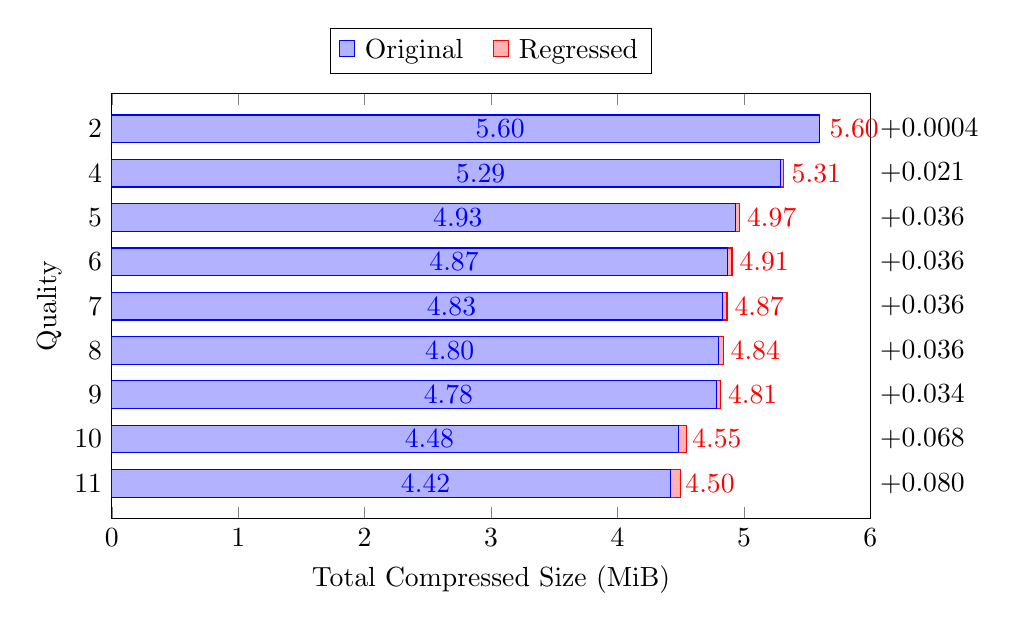
\begin{tikzpicture}
\begin{axis}[
	width = 0.925\textwidth,
	height = 0.96*\axisdefaultheight,
	xbar stacked,
	xmin = 0,
	xmax = 6,
	xtick distance = 1,
	y dir = reverse,
	ytick = data,
	ytick pos = left,
	yticklabels = {2, 4, 5, 6, 7, 8, 9, 10, 11},
	extra y ticks = {0, 1, 2, 3, 4, 5, 6, 7, 8},
	extra y tick labels = {$+0.0004$, $+0.021$, $+0.036$, $+0.036$, $+0.036$, $+0.036$, $+0.034$, $+0.068$, $+0.080$},
	extra y tick style = {ticklabel pos = right},
	scaled ticks = false,
	enlarge x limits = {abs = 0},
	enlarge y limits = {abs = 0.8},
	nodes near coords,
	nodes near coords align = {horizontal},
	nodes near coords style = {/pgf/number format/.cd, fixed zerofill, precision = 2},
	legend columns = -1,
	legend style = {
		at = {(0.5, 1.045)},
		anchor = south,
		column sep = 0.05cm,
		/tikz/every even column/.append style = {
			column sep = 0.3cm
		}
	},
	legend image code/.code = {
		\draw[#1] (0cm, -0.075cm) rectangle (0.2cm, 0.135cm);
	},
	xlabel = Total Compressed Size (MiB),
	ylabel = Quality,
	ylabel style = {yshift = -width(+0.0000)}
]
\legend{
	Original,
	Regressed,
	Improved
}
\addplot[blue, fill = blue!30!white] coordinates {
	(5.60, 0)
	(5.29, 1)
	(4.93, 2)
	(4.87, 3)
	(4.83, 4)
	(4.80, 5)
	(4.78, 6)
	(4.48, 7)
	(4.42, 8)
};
\addplot[red, fill = red!30!white, point meta = x] coordinates {
	(0.0004, 0)
	(0.0210, 1)
	(0.0356, 2)
	(0.0355, 3)
	(0.0357, 4)
	(0.0355, 5)
	(0.0344, 6)
	(0.0678, 7)
	(0.0801, 8)
};
\end{axis}
\end{tikzpicture}